\documentclass[10pt]{article}
\usepackage[margin=0.7in]{geometry}
\usepackage[T1]{fontenc}
\usepackage{graphicx,hyperref}
\begin{document}
\sloppy
\section*{Native quotient word-storage bridge}
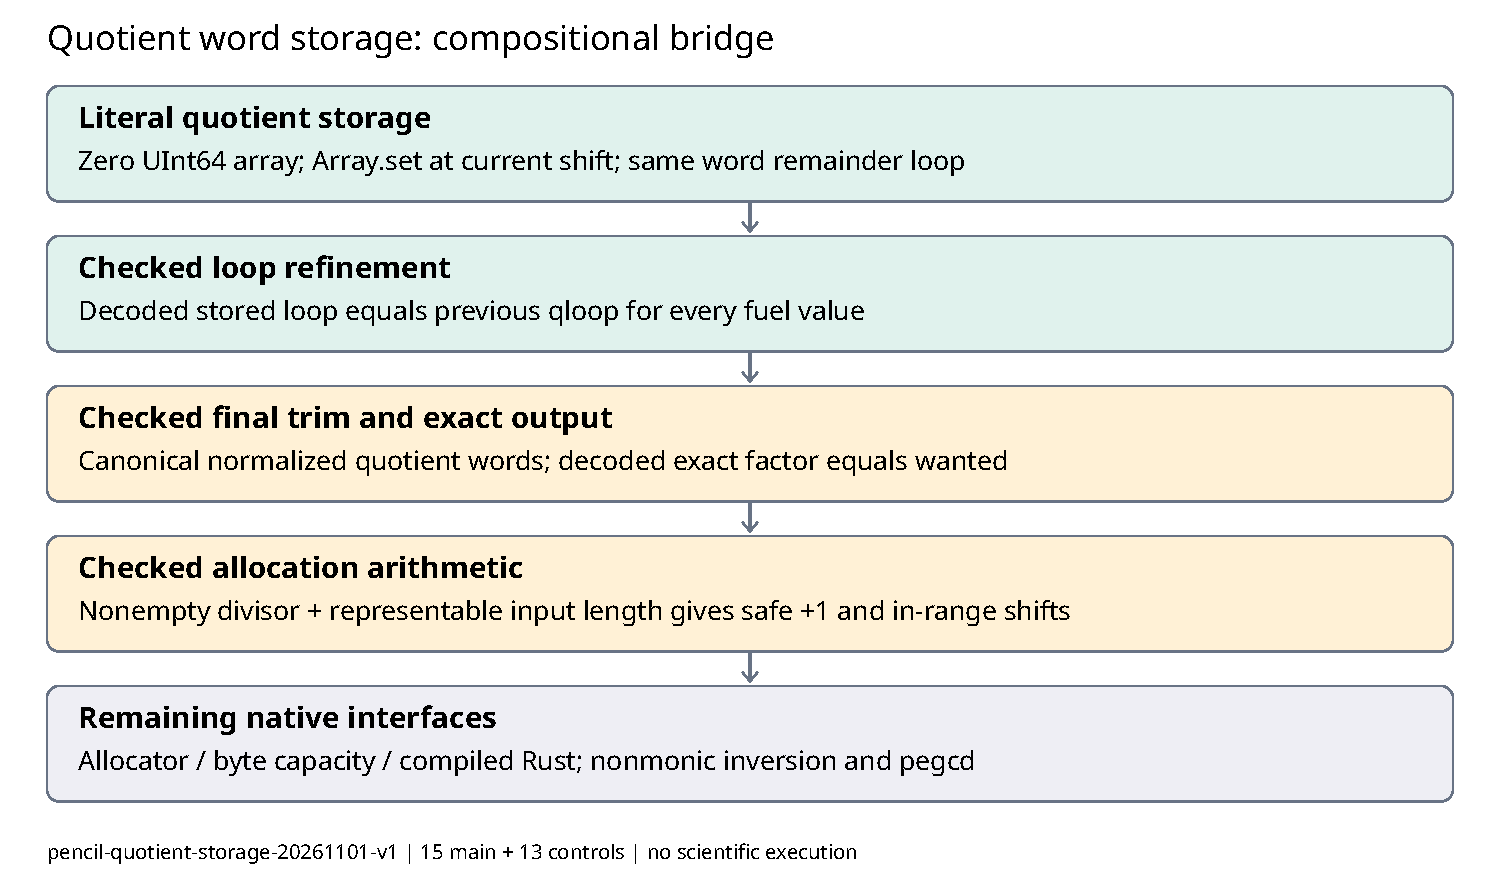
\includegraphics[width=\linewidth]{flow.pdf}
Fifteen main declarations and thirteen controls passed, with twenty-eight exact named axiom readbacks. The division quotient now has an executable word-storage model: zero-initialized Array UInt64, indexed overwrites of the selected remainder word, the existing word-remainder step, and final quotient trimming. A whole-loop refinement connects it to checkedDiv and the prior exact-quotient theorem; this is more than an isolated setter identity.\par\medskip
Source and prior-review basis. Native three\_leads.rs849-880 initializes q with a.len().saturating\_sub(b.len())+1 zero words, assigns q[j]=c, updates and trims the remainder, and returns trim(q). The prior independent division review explicitly identified the quotient Vec, trim and usize allocation as remaining interfaces. That review and the native source were inspected before the new PLAN and proof code. This packet retains the monic branch: final divisor word1, inverse-leading value1, shift r.length-b.length, and multiplier r.getLast. Nonmonic inversion and general pegcd are separate.\par\medskip
Storage and decoding. QuotientStorage.put uses Array.set on a typed in-range index. put\_good preserves canonical words, and put\_decode proves that decoding the resulting array equals the earlier polynomial writeCoeff operation. That operation replaces exactly one coefficient and leaves all others unchanged, including repeated writes. Initial storage reuses the checked zero-array constructor, canonicality and zero-polynomial theorem. No list of supplied quotient coefficients is substituted for the actual array writes.\par\medskip
Whole-loop composition. wloop carries a fixed-size UInt64 array and executes the same selected remainder traversal and trim as the prior model. An explicit index guard rejects out-of-bounds states. loop\_refines proves that under the original-input length bound and sufficient allocated quotient slots, this guard always admits every active step and the decoded entire stored loop equals qloop for every fuel value. Strict remainder shortening maintains the bound across recursion. loop\_good proves canonical quotient storage and remainder preservation. The prior fresh-slot invariant and Q*B+R theorem therefore apply through this proved refinement rather than being re-assumed for the array.\par\medskip
Final trim and exact result. finish trims the array's coefficient list; finish\_decode preserves its polynomial, finish\_good preserves canonicality, and finish\_normal proves no trailing zero word remains. word\_projection identifies the decoded final wordDiv result with checkedDiv, including failure/insufficient-fuel outcomes. word\_success gives A=Q*B+R and the terminal remainder bound. word\_total derives success at input-length fuel. word\_exact composes returns\_given\_exact: from a decoded factorization A=wanted*B it produces actual quotient words q with wordDiv=some(q,[]), Canon q, and wordsPoly(q)=wanted. word\_normal additionally applies to every successful output. This is the storage endpoint for the CZero quotient X-x.\par\medskip
Allocation arithmetic. allocation\_bound proves for any positive word width w that a<2\textasciicircum{}w and nonempty divisor length b imply a-b+1<2\textasciicircum{}w, where subtraction is saturating natural subtraction. current\_index\_bound proves every current shift r-b is inside the allocated capacity given r<=a and a-b<capacity. The 64-bit boundary control tests a=2\textasciicircum{}64-1 and b=1; a separate b=0 counterexample demonstrates why the native nonempty-divisor assertion is necessary for this +1 bound. These are representability and index certificates. They do not establish physical allocation success, Vec byte-layout/isize limits, allocator behavior, or a compiled Rust execution trace.\par\medskip
Controls. Kernel-checked executable cases cover empty input, an all-zero input, empty divisor rejection, exact quotient[1,1] for [16,0,1]/[16,1] over modulus17, nonexact remainder[2], leading zeros in the input and allocated quotient, division by constant1, insufficient fuel, repeated overwrite of a used slot, a zero-capacity guard, both allocation arithmetic boundaries and positivity of the native capacity formula. Leading-zero inputs produce the same trimmed quotient words. Zero-capacity is an intentionally invalid internal state; the actual initialization allocates at least one slot. No large array is allocated for the 64-bit arithmetic controls.\par\medskip
Checks and assumptions. Final gates storage1, loop1, division2, endpoint1, controls1 and readback1 passed with unchanged input bindings. Exact named inventory acceptance covers fifteen main declarations and thirteen controls; only propext, Classical.choice and Quot.sound occur. The initial division1 proof failed on equality transport/projection syntax and was repaired; its original source and receipt remain. Prime p, 0<p<2\textasciicircum{}31 and canonical input words are proof premises; admission tests monicity, not runtime canonicality. General arithmetic, remainder descent and normalization are imported from the existing checked components. The helper binds direct source and compiled roots; transitive cached binaries and the Lean compiler remain trusted without an independent binary kernel rechecker.\par\medskip
Scope and next integration. The natural-number allocation and index bounds plus the literal UInt64 Array.set/trim model close the previous quotient-storage abstraction at the Lean model level. Rust allocator/resource exceptions, usize implementation refinement, instrumentation, native nonmonic division, general pegcd and compiled equivalence are not claimed. This producer packet awaits publication and independent review under T-1237. It preserves the 1,260-target campaign scope and expired scientific limits. No scientific execution, cloud action or repository edit occurred.\par\medskip
\end{document}